\documentclass [a4paper] {article}
\usepackage[hidelinks]{hyperref}
\usepackage[spanish,activeacute]{babel}
\usepackage[utf8]{inputenc}
\usepackage{amsmath}
\usepackage{graphicx}
\usepackage{tikz}
\usepackage{booktabs}

\setlength{\parindent}{0pt}
\textwidth = 500pt
\hoffset = -70pt

\title{\textbf{Fundamentos de la Ciencia de Datos Práctica 4}}
\author{
	Fernández Díaz, Daniel\\
	Cano Díaz, Francisco\\
	Fernández Hernández, Alberto\\
}

\date{19 de noviembre del 2019}
\usepackage{Sweave}
\begin{document}
\input{G15-P4-concordance}
\maketitle
\newpage
\tableofcontents
\newpage
\section{Apartado 1}
En este apartado se resolverá el problema visto en teoría realizando un análisis de clasificación no supervisada con R tal y como vimos en clase. Por último, se realizará el proceso paso a paso de forma similar a la vista en teoría para comprobar que ambos resultados coinciden.
\subsection{Algoritmo K-means en R}
\subsubsection{Obtención de los datos}
En primer lugar, leeremos los datos de los puntos y los centroides iniciales del fichero \textbf{\textit{apartado1.txt}} utilizando la función \textbf{muestra.leer} desarrollada para la práctica 3, la cual permite leer varias tablas o data frames de un mismo archivo.
\begin{footnotesize}

\begin{Schunk}
\begin{Sinput}
> muestra <- muestra.leer("apartado1.txt")
> m_clasif <- muestra[[1]]
> c_clasif <- muestra[[2]]
\end{Sinput}
\end{Schunk}
\end{footnotesize}
De esta forma cargamos nuestra matriz de clasificaciones como un data frame llamado \textbf{m\_clasif}:
\begin{Schunk}
\begin{Soutput}
  d1 d2
1  4  4
2  3  5
3  1  2
4  5  5
5  0  1
6  2  2
7  4  5
8  2  1
\end{Soutput}
\end{Schunk}

Y otro dataframe llamado \textbf{c\_clasif} con las coordenadas iniciales de nuestros centroides, que en este caso son dos:
\begin{Schunk}
\begin{Soutput}
  d1 d2
1  0  1
2  2  2
\end{Soutput}
\end{Schunk}

\subsubsection{Ejecución del algoritmo}
Con esto, ya podemos ejecutar la función \textbf{\textit{kmeans}} donde además de los dos data frames ya mencionados, le pasamos como tercer argumento un 4, que indica el número de iteraciones máximas que permitimos al algoritmo. Este parámetro es importante ya que el algoritmo puede no converger. Por último mencionar que típicamente se le pasan a esta función dos matrices, una con los puntos y otra con los centroides; pero funciona igual con data frames (los convierte internamente) por lo que no es necesario que nossotros hagamos esa conversión previamente.
\vspace{5mm}
\begin{Schunk}
\begin{Sinput}
> (clasif_ns <- kmeans(m_clasif,c_clasif,4))
\end{Sinput}
\begin{Soutput}
K-means clustering with 2 clusters of sizes 4, 4

Cluster means:
    d1   d2
1 1.25 1.50
2 4.00 4.75

Clustering vector:
1 2 3 4 5 6 7 8 
2 2 1 2 1 1 2 1 

Within cluster sum of squares by cluster:
[1] 3.75 2.75
 (between_SS / total_SS =  84.8 %)

Available components:

[1] "cluster"      "centers"      "totss"        "withinss"     "tot.withinss"
[6] "betweenss"    "size"         "iter"         "ifault"      
\end{Soutput}
\end{Schunk}

\subsubsection{Resultados}
Como resultado, obtenemos una estructura de datos con toda la información calculada por el algoritmo: un data frame con las coordenadas finales de los centroides, un vector de asociaciones, etc.

En ese vector de asociaciones o \textit{clustering vector} figura la clase a la que pertenece cada uno de los puntos; y es precisamente este vector el que utilizaremos en un último paso para dividir los datos iniciales y extraer información del análisis. Para ello añadimos dicho vector como columna a la estructura de datos que contenía los puntos:
\begin{Schunk}
\begin{Sinput}
> cluster <- clasif_ns$cluster
> (m_clasif <- cbind(cluster,m_clasif))
\end{Sinput}
\begin{Soutput}
  cluster d1 d2
1       2  4  4
2       2  3  5
3       1  1  2
4       2  5  5
5       1  0  1
6       1  2  2
7       2  4  5
8       1  2  1
\end{Soutput}
\end{Schunk}
Y dividimos dicha estructura en dos, cada una con los puntos de cada cluster:
\begin{Schunk}
\begin{Sinput}
> m_c1 <- subset(m_clasif,m_clasif[,1]==1)
> (m_c1 <- m_c1[,-1])
\end{Sinput}
\begin{Soutput}
  d1 d2
3  1  2
5  0  1
6  2  2
8  2  1
\end{Soutput}
\begin{Sinput}
> m_c2 <- subset(m_clasif,m_clasif[,1]==2)
> (m_c2 <- m_c2[,-1])
\end{Sinput}
\begin{Soutput}
  d1 d2
1  4  4
2  3  5
4  5  5
7  4  5
\end{Soutput}
\end{Schunk}


\section{Apartado 2}
\subsection{Programación de nuestro propio \textbf{k-means}}
\subsubsection{El código}
En este apartado presentaremos el algoritmo \textbf{k-means} que hemos programado siguiendo los pasos vistos en la teoría. El código es el siguiente:
\begin{footnotesize}
\begin{Schunk}
\begin{Sinput}
> our.kmeans <- function(muestra,centroides,aleatorio=TRUE){
+   if(aleatorio) centroides = elegir.centroides(muestra,centroides)
+ 
+   continuar = TRUE
+   asignacion.old = matrix(0,nrow=nrow(centroides),ncol=nrow(muestra))
+ 
+   while(continuar){
+     distancias = crear.matriz.distancias(muestra,centroides)
+     asignacion = crear.matriz.asignacion(distancias)
+     centroides = crear.centroides(muestra,distancias,asignacion)
+ 
+     if(comprobar.matriz.asignacion(asignacion,asignacion.old)) continuar = FALSE
+     else asignacion.old = asignacion
+   }
+ 
+   vector.clusters = crear.vector.clusters(asignacion)
+   list(m.distancias=distancias,m.asignacion=asignacion,centroides=centroides,v.clusteriz=vector.clusters)
+ }
> ## Distancia euclidea ##
> # Calcula la distancia euclidea entre dos puntos.
> distancia.euclidea <- function(p1,p2){
+   sum = 0
+   for(i in 1:length(p1)){
+   	sum = sum + ((p1[1,i] - p2[1,i])^2)
+   }
+   sqrt(sum)
+ }
> ## Seleccion de centroides de forma aleatoria ##
> # A partir de la muestra utilizada para el K-MEANS obtiene
> # los centroides de forma aleatoria a partir de los puntos
> # que conforman la muestra.
> elegir.centroides <- function(muestra,num.centroides){
+   if(num.centroides > nrow(muestra)){
+   	num.centroides <- nrow(muestra)
+   } else if(num.centroides < 1){
+   	num.centroides <- 1
+   }
+   
+   centroides = matrix(nrow=0,ncol=ncol(muestra))
+   
+   # Obtenemos cada uno de los centroides. Estos centroides seran,
+   # de forma aleatoria, algunos o todos los puntos de la muestra.
+   for(i in 1:num.centroides){
+     centroide = floor(runif(1,min=1,max=nrow(muestra)))
+     centroides = rbind(centroides,muestra[centroide,])
+     muestra = muestra[-centroide,]
+   }
+   colnames(centroides) <- c(paste0("d",1:ncol(centroides)))
+   rownames(centroides) <- c(paste0("C",1:nrow(centroides)))
+   as.data.frame(centroides)
+ }
> ## Creacion de la matriz de distancias ##
> # Obtenemos en forma de matriz la distancia de cada uno de
> # los puntos de la muestra a cada uno de los centroides definidos.
> crear.matriz.distancias <- function(muestra,centroides){
+   vd = c()
+   md = matrix(nrow=0,ncol=nrow(muestra))
+   for(i in 1:nrow(centroides)){
+     # Obtenemos las coordenadas del centroide correspondiente.
+     c = centroides[i,]
+     for(j in 1:nrow(muestra)){
+       # Obtenemos las coordenadas del punto correspondiente.
+       m = muestra[j,]
+       # Calculamos la distancia entre ambos y la añadimos al vector.
+       vd = c(vd,distancia.euclidea(m,c))
+     }
+     md = rbind(md,vd)
+     vd = c()
+   }
+   colnames(md) = c(paste0("P",1:nrow(muestra)))
+   rownames(md) = c(paste0("C",1:nrow(centroides)))
+   as.data.frame(md)
+ }
> ## Creacion de la matriz de asignacion ##
> # Obtenemos en forma de matriz la pertenencia de cada punto
> # de la muestra a cada cluster de tal forma que se indicara
> # con un 1 aquellos puntos que pertenezcan y un 0 a aquellos
> # que no.
> crear.matriz.asignacion <- function(distancias){
+   #Creamos la matriz de asignacion con valores a 0
+   ma = matrix(0,nrow=nrow(distancias),ncol=ncol(distancias))
+   rownames(ma) = c(paste0("C",1:nrow(distancias)))
+   colnames(ma) = c(paste0("P",1:ncol(distancias)))
+ 
+   for(i in 1:ncol(distancias)){
+     # Obtiene el indice del menor valor del punto correspondiente.
+     # Este punto sera asignado al cluster mas cercano.
+     indice.menor = which.min(distancias[,i])
+ 
+     #Por tanto el valor de ese puto para ese cluster sera 1: pertenece
+     ma[indice.menor,i] = 1
+   }
+ 
+   # Una vez tenemos el vector con las asignaciones lo convertimos a dataframe.
+   as.data.frame(ma)
+ }
> ## Creacion de los nuevos centroides ##
> # Obtenemos los nuevos centroides a partir de los nuevos
> # puntos obtenidos en la matriz de asignacion. Para ello
> # calculamos el promedio de cada coordenada obteniendo asi
> # las coordenadas de cada uno de los centroides.
> crear.centroides <- function(muestra,distancias,asignacion){
+   puntos = matrix(nrow=0,ncol=ncol(muestra))
+   centroides = matrix(nrow=0,ncol=ncol(muestra))
+ 
+   for(i in 1:nrow(asignacion)){
+     for(j in 1:ncol(asignacion)){
+       # Para los puntos que pertenecen a cada cluster,
+       # obtenemos la coordenada x e y de todos ellos.
+       if(asignacion[i,j] == 1){
+         puntos = rbind(puntos,muestra[j,])
+       }
+     }
+     # Obtenemos el nuevo centroide mediante la media de las
+     # coordenadas.
+     centroides = rbind(centroides,calcular.centroide(puntos))
+     puntos = matrix(nrow=0,ncol=ncol(muestra))
+   }
+ 
+   # Una vez tenemos el vector con los centroides lo convertimos a dataframe.
+   rownames(centroides) = c(paste0("C",1:nrow(centroides)))
+   colnames(centroides) = c(paste0("d",1:ncol(centroides)))
+   as.data.frame(centroides)
+ }
> ## Calculo de las coordenadas del centroide ##
> # Se calculan las coordenadas del centroide a partir de la 
> # media de los puntos de su cluster
> calcular.centroide <- function(puntos){
+   centroide = c()
+   sum = 0
+ 
+   # Calculo de la media de cada coordenada o dimension de los puntos
+   for(i in 1:ncol(puntos)){
+     for(j in 1:nrow(puntos)){
+       sum = sum + puntos[j,i]
+     }
+     centroide = c(centroide,sum/nrow(puntos))
+     sum = 0
+   }
+   centroide
+ }
> ## Condicion de parada ##
> # Indica al algoritmo si debe parar atendiendo a la comparacion de
> # la matriz de asignacion anterior y la nueva. Si no cambia
> # (iguales=TRUE) significa que los centroides no se han movido en
> # esta iteracion y podemos parar
> comprobar.matriz.asignacion <- function(asignacion.antigua, asignacion.nueva){
+   iguales = asignacion.antigua == asignacion.nueva
+   iguales = all(iguales)
+ }
> ## Creacion del vector de clusterizacion ##
> crear.vector.clusters <- function(asignacion){
+   mc = matrix(nrow=1,ncol=ncol(asignacion))
+   rownames(mc) = "C"
+   colnames(mc) = c(paste0("P",1:ncol(asignacion)))
+ 
+   for(i in 1:ncol(asignacion)){
+     for(j in 1:nrow(asignacion)){
+       if(asignacion[j,i]) mc[1,i] = j
+     }
+   }
+ 
+   as.data.frame(mc)
+ }
> ## Grafica de los resultados (2D)##
> # Muestra los puntos sobre el plano X-Y, asi como los centroides
> # y los clusters obtenidos
> plot2D.our.kmeans <- function(muestra,kmeans){
+   # Nos aseguramos de que el imput sea 2D
+   if(ncol(muestra)!=2) stop("Dimensiones erroneas. Asegurate de que las estructuras son de 2D")
+   
+   # Estructura aux con vector de clusterizacion, muestra y matriz de distancias
+   aux = cbind(C=t(kmeans$v.clusteriz),muestra=muestra,dist=t(kmeans$m.distancias))
+ 
+   # Calculo del rango del plot
+   rango.x = range(aux$muestra.d1); rango.y = range(aux$muestra.d2)
+   centroide.min = centroide.minimo(kmeans$centroides,rango.x,rango.y) # Etiqueta del centroide min
+   centroide.max = centroide.maximo(kmeans$centroides,rango.x,rango.y) # Etiqueta del centroide max
+   clusters = crear.clusters(aux,nrow(kmeans$centroides)) # Datos clusterizados
+ 
+   rango.x = c(min(kmeans$centroides[centroide.min,][1]-max(clusters[[centroide.min]][paste0("dist.",centroide.min)]),rango.x[1]),
+     max(kmeans$centroides[centroide.max,][1]+max(clusters[[centroide.max]][paste0("dist.",centroide.max)]),rango.x[2]))
+   rango.y = c(min(kmeans$centroides[centroide.min,][2]-max(clusters[[centroide.min]][paste0("dist.",centroide.min)]),rango.y[1]),
+     max(kmeans$centroides[centroide.max,][2]+max(clusters[[centroide.max]][paste0("dist.",centroide.max)]),rango.y[2]))
+ 
+   # Plot centroides
+   plot(kmeans$centroides,pch=22,col='blue',xlim=rango.x,ylim=rango.y)
+   etiquetas = c("Centroides"); puntos = c(22); linea = c(0); color = c(4)
+ 
+   for(i in 1:length(clusters)){
+     # Plot puntos
+     points(clusters[[paste0("C",i)]]$muestra.d1,clusters[[paste0("C",i)]]$muestra.d2,pch=19,col=i)
+     etiquetas = c(etiquetas,paste0("Cluster ",i)); puntos = c(puntos,19); linea = c(linea,0); color = c(color,i)
+ 
+     # Plot contorno actual del cluster
+     symbols(kmeans$centroides[paste0("C",i),'d1'],kmeans$centroides[paste0("C",i),'d2'],
+       circle=0.1+max(clusters[[paste0("C",i)]][paste0("dist.C",i)]),add=TRUE,inches=FALSE)
+     etiquetas = c(etiquetas,paste0("Frontera ",i)); puntos = c(puntos,46); linea = c(linea,1); color = c(color,1)
+   }
+ 
+   # Titulo
+   title(sprintf("Clusterizacion K-means con %i clusters",length(clusters)))
+   # Leyenda
+   legend(rango.x[1], rango.y[2], legend=etiquetas, lty=linea, pch = puntos, col = color, cex=0.8)
+ }
> ## Calcular el centroide minimo ##
> # Calcula cual es el centroide con la distancia mas cercana al limite inferior del rango del plot
> centroide.minimo <- function(centroides,rango.x,rango.y){
+   distancias = c()
+   for(i in 1:nrow(centroides)){
+     distancias = c(distancias,distancia.euclidea(centroides[i,],matrix(c(rango.x[1],rango.y[1]),nrow=1)))
+   }
+   rownames(centroides[(order(distancias)[1]),])
+ }
> ## Calcular el centroide maximo ##
> # Calcula cual es el centroide con la distancia mas cercana al limite superior del rango del plot
> centroide.maximo <- function(centroides,rango.x,rango.y){
+   distancias = c()
+   for(i in 1:nrow(centroides)){
+     distancias = c(distancias,distancia.euclidea(centroides[i,],matrix(c(rango.x[2],rango.y[2]),nrow=1)))
+   }
+   rownames(centroides[(order(distancias)[1]),])
+ }
> ## Crear clusters ##
> # Dado un conjunto de datos con un vector de clusterizacion en una de las
> # columnas, agrupa los datos en grupos en funcion de a que cluster pertenece
> # cada punto y devulve una lista de dichos puntos
> crear.clusters <- function(datos,num.clusters){
+   grupos = list()
+   for(i in 1:num.clusters){
+     grupos[[paste0("C",i)]] = subset(datos,datos$C==i)
+   }
+   grupos
+ }
\end{Sinput}
\end{Schunk}
\end{footnotesize}

\newpage
\subsubsection{Ejemplo de ejecución en 2D}
La función principal de nuestro algoritmo es \textbf{\textit{our.kmeans(muestra,centroides,aleatorio)}}, donde:
\begin{itemize}
\item \textbf{muestra} son los puntos a clusterizar
\item \textbf{centroides} puede ser:
	\begin{itemize}
	\item un dataframe con las coordenadas de los centroides que queremos utilizar en esa clusterizacion. Para ello el parametro aleatorio debe estar a FALSE, indicando al programa que no se desean coordenadas aleatorias para los centroides iniciales.
	\item un entero, el numero de clusters en el que se desean dividir los datos. Para ello el parametro aleatorio debe estar a TRUE, indicando al programa que se desean coordenadas aleatorias para los centroides iniciales.
	\end{itemize}
\item \textbf{aleaorio} es una variable logica con valor TRUE por defecto. Indica al programa si se desean o no coordenadas aleatorias para los centroides iniciales.
\end{itemize}

Si ejecutamos la función con los datos del apartado 1 (muestra y centroides) obtenemos unos resultados muy similares al algoritmo de el paquete \textit{stats} de CRAN:
\begin{Schunk}
\begin{Sinput}
> m_clasif <- muestra[[1]]
> c_clasif <- muestra[[2]]
> (km <- our.kmeans(m_clasif,c_clasif,F))
\end{Sinput}
\begin{Soutput}
$m.distancias
         P1       P2       P3       P4       P5        P6       P7        P8
C1 3.716517 3.913119 0.559017 5.129571 1.346291 0.9013878 4.451123 0.9013878
C2 0.750000 1.030776 4.069705 1.030776 5.482928 3.4003676 0.250000 4.2500000

$m.asignacion
   P1 P2 P3 P4 P5 P6 P7 P8
C1  0  0  1  0  1  1  0  1
C2  1  1  0  1  0  0  1  0

$centroides
     d1   d2
C1 1.25 1.50
C2 4.00 4.75

$v.clusteriz
  P1 P2 P3 P4 P5 P6 P7 P8
C  2  2  1  2  1  1  2  1
\end{Soutput}
\end{Schunk}

\newpage
\subsubsection{Ejemplo de ejecucion en 3D}
Este algoritmo funciona también con puntos de más de dos dimensiones. Veamos un pequeño ejemplo: cojamos los puntos de la muestra original que acabamos de utilizar y añadamosle una tercera dimensión pero manteniendo los puntos en un mismo plano, de forma que no perdamos la agrupación original de estos. El algoritmo \textbf{K-means} solo funciona bien con puntos claramente agrupados.
\begin{Schunk}
\begin{Sinput}
> (m3 <- cbind(muestra[[1]],d3=(1:8)/4))
\end{Sinput}
\begin{Soutput}
  d1 d2   d3
1  4  4 0.25
2  3  5 0.50
3  1  2 0.75
4  5  5 1.00
5  0  1 1.25
6  2  2 1.50
7  4  5 1.75
8  2  1 2.00
\end{Soutput}
\begin{Sinput}
> our.kmeans(m3,2)
\end{Sinput}
\begin{Soutput}
$m.distancias
          P1       P2        P3       P4       P5        P6        P7       P8
C1 3.8830561 4.009754 0.8385255 5.143260 1.352082 0.9100137 4.4668921 1.096871
C2 0.9762812 1.096871 4.0716244 1.038328 5.495737 3.4573292 0.9100137 4.396376

$m.asignacion
   P1 P2 P3 P4 P5 P6 P7 P8
C1  0  0  1  0  1  1  0  1
C2  1  1  0  1  0  0  1  0

$centroides
     d1   d2    d3
C1 1.25 1.50 1.375
C2 4.00 4.75 0.875

$v.clusteriz
  P1 P2 P3 P4 P5 P6 P7 P8
C  2  2  1  2  1  1  2  1
\end{Soutput}
\end{Schunk}

Como podemos ver, al estar todos en un mismo plano los clusters solucion se mantienen inalterados aunque con una dimensión más.

\newpage
\subsubsection{Visualización de los resultados}
Además, hemos creado también una función \textbf{\textit{plot2D.our.kmeans(muestra,kmeans)}} con los siguientes parámetros:
\begin{itemize}
\item \textbf{muestra} es la muestra inicial utilizada en el algoritmo \textbf{k-means}
\item \textbf{kmeans} es la estructura (lista) devuelta por dicho algoritmo
\end{itemize}

Esta función solo sirve para puntos en \textbf{dos dimensiones}. Dados dichos puntos y la información de la clusterizacion obtenida de la estructura kmeans, realiza un plot de dichos puntos agrupados en sus respectivos clusters (dibujados con diferente color para cada cluster); así como los centroides de dichos clusters y una especie de frontera imaginaria del cluster que contiene los puntos que lo conforman hasta el momento. Este círculo no tiene valor analítico pero se ha considerado incluirlo en estas gráficas de ejemplo para hacer la clusterización más visual. En un estudio serio, estos círculos se quitarían.

Veamos ahora algunos ejemplos con los puntos originales en 2D y con una división en 2, 3, 4, 5 y 6 clusters:
\begin{figure}[htbp!]
\centering
\begin{Schunk}
\begin{Sinput}
> plot2D.our.kmeans(m_clasif,our.kmeans(m_clasif,2))
\end{Sinput}
\end{Schunk}
\includegraphics{G15-P4-011}
\caption{División en 2 clusters}
\end{figure}

\begin{figure}[htbp!]
\centering
\begin{Schunk}
\begin{Sinput}
> plot2D.our.kmeans(m_clasif,our.kmeans(m_clasif,3))
\end{Sinput}
\end{Schunk}
\includegraphics{G15-P4-012}
\caption{División en 3 clusters}
\end{figure}

\begin{figure}[htbp!]
\centering
\begin{Schunk}
\begin{Sinput}
> plot2D.our.kmeans(m_clasif,our.kmeans(m_clasif,4))
\end{Sinput}
\end{Schunk}
\includegraphics{G15-P4-013}
\caption{División en 4 clusters}
\end{figure}

\begin{figure}[htbp!]
\centering
\begin{Schunk}
\begin{Sinput}
> plot2D.our.kmeans(m_clasif,our.kmeans(m_clasif,5))
\end{Sinput}
\end{Schunk}
\includegraphics{G15-P4-014}
\caption{División en 5 clusters}
\end{figure}

\begin{figure}[htbp!]
\centering
\begin{Schunk}
\begin{Sinput}
> plot2D.our.kmeans(m_clasif,our.kmeans(m_clasif,6))
\end{Sinput}
\end{Schunk}
\includegraphics{G15-P4-015}
\caption{División en 6 clusters}
\end{figure}

\newpage
\subsection{Análisis del número de \textit{clusters} óptimos. Comparación K-Means y \textit{Hierarchical Clustering}. Algoritmo DBSCAN}
\subsubsection{K-Means}
Vamos a realizar una modificación del ejercicio de clase, en el \textbf{visualizaremos puntos de acceso \textit{Wi-Fi}}, agrupando los diferentes puntos mediante \textit{K-Means}. Para ello utilizaremos un \textit{dataset} geográfico con los puntos de acceso \textit{Wi-Fi} de la ciudad de Nueva York. \footnote{\url{https://data.cityofnewyork.us/api/views/varh-9tsp/rows.csv?accessType=DOWNLOAD}} Para visualizar los datos, utilizaremos la librería \textit{dplyr}, el cual nos permite manipular un \textit{dataframe} de forma similar a una consulta \texttt{SQL}.
\begin{footnotesize}
\begin{Schunk}
\begin{Sinput}
> # Incluimos la libreria dplyr
> if(!require(dplyr)){
+   install.packages("dplyr")
+   require(dplyr)
+ }
\end{Sinput}
\begin{Soutput}
--- Please select a CRAN mirror for use in this session ---

  There is a binary version available but the source version is later:
      binary source needs_compilation
rlang  0.4.1  0.4.2              TRUE

  Binaries will be installed
package ‘rlang’ successfully unpacked and MD5 sums checked
package ‘dplyr’ successfully unpacked and MD5 sums checked

The downloaded binary packages are in
	C:\Users\solol\AppData\Local\Temp\RtmpCgG4GG\downloaded_packages
\end{Soutput}
\begin{Sinput}
> # Preparamos el dataframe
> newyork <- read.csv("NYC_Free_Public_WiFi_03292017.csv")
> # Similar a la consulta SQL:
> # SELECT * FROM newyork LIMIT 5
> newyork %>% head(5)
\end{Sinput}
\begin{Soutput}
  BORO                                     the_geom OBJECTID TYPE             PROVIDER         NAME               LOCATION      LAT       LON       X        Y    LOCATION_T                                          REMARKS     CITY
1   BK POINT (-73.87053740957452 40.68406083967918)    10321 Free LinkNYC - Citybridge bk-05-145941     3386 FULTON STREET 40.68406 -73.87054 1020156 188524.8 Outdoor Kiosk Tablet Internet -phone , Free 1 GB Wi-FI Service Brooklyn
2   BK POINT (-73.86897452703059 40.68462509021575)    10322 Free LinkNYC - Citybridge bk-05-145940     3435 FULTON STREET 40.68463 -73.86897 1020589 188731.0 Outdoor Kiosk Tablet Internet -phone , Free 1 GB Wi-FI Service Brooklyn
3   BK POINT (-73.86830878947508 40.68470155389536)    10323 Free LinkNYC - Citybridge bk-05-145939     3450 FULTON STREET 40.68470 -73.86831 1020774 188759.1 Outdoor Kiosk Tablet Internet -phone , Free 1 GB Wi-FI Service Brooklyn
4   BK POINT (-73.86677732990765 40.68513094043811)    10324 Free LinkNYC - Citybridge bk-05-145938     3480 FULTON STREET 40.68513 -73.86678 1021198 188916.2 Outdoor Kiosk Tablet Internet -phone , Free 1 GB Wi-FI Service Brooklyn
5   BK POINT (-73.89716745051707 40.67647466963193)    10325 Free LinkNYC - Citybridge bk-05-145932 62 PENNSYLVANIA AVENUE 40.67647 -73.89717 1012774 185751.1 Outdoor Kiosk Tablet Internet -phone , Free 1 GB Wi-FI Service Brooklyn
                SSID    SOURCEID                    ACTIVATED BOROCODE BORONAME NTACODE                 NTANAME COUNDIST POSTCODE BOROCD CT2010 BOROCT2010     BIN        BBL DOITT_ID
1 LinkNYC Free Wi-Fi LINK-021921 11/21/2017 12:00:00 AM +0000        3 Brooklyn    BK83 Cypress Hills-City Line       37    11208    305    184    3118400 3327234 3041480040     4726
2 LinkNYC Free Wi-Fi LINK-021922 11/21/2017 12:00:00 AM +0000        3 Brooklyn    BK83 Cypress Hills-City Line       37    11208    305    184    3118400 3092471 3041340160     4727
3 LinkNYC Free Wi-Fi LINK-021923 11/21/2017 12:00:00 AM +0000        3 Brooklyn    BK83 Cypress Hills-City Line       37    11208    305    184    3118400 3093023 3041510030     4728
4 LinkNYC Free Wi-Fi LINK-021925 12/20/2017 12:00:00 AM +0000        3 Brooklyn    BK83 Cypress Hills-City Line       37    11208    305    184    3118400 3093078 3041520030     4729
5 LinkNYC Free Wi-Fi LINK-021926 02/06/2018 12:00:00 AM +0000        3 Brooklyn    BK82           East New York       37    11207    305    198    3119800 3083275 3036690030     4730
\end{Soutput}
\end{Schunk}
\end{footnotesize}

El \textit{dataframe} contiene, entre otros campos, los siguientes atributos:
\begin{enumerate}
  \item \textit{BORO}: barrio de la ciudad (ejemplo: BK = \textit{Brooklyn}).
  \item \textit{the\_geom}: coordenadas de latitud y longitud.
  \item \textit{OBJECTID}: id del punto de conexión.
  \item \textit{TYPE}: tipo de red (\textit{free, limited-free...})
  \item \textit{PROVIDER}: nombre del proveedor.
  \item \textit{NAME}: nombre de la red.
  \item \textit{LOCATION}: localización.
  \item \textit{LAT}: latitud.
  \item \textit{LON}: longitud.
\end{enumerate}

Para aplicar el algoritmo \textit{K-Means}, utilizaremos únicamente los atributos \textit{LAT} y \textit{LON}:
\begin{Schunk}
\begin{Sinput}
> newyork.df <- data.frame(newyork$LAT, newyork$LON)
\end{Sinput}
\end{Schunk}

Una vez tengamos estas columnas, vamos a determinar el número de \textit{clusters} óptimos. Para ello vamos a trabajar con dos algoritmos básicos:
\begin{itemize}
  \item \textit{Elbow Method}
  \item \textit{Average Silhouette Method}
\end{itemize}

\paragraph{Elbow Method}: 
El objetivo de este algoritmo es \textbf{minimizar la suma de los cuadrados de las distancias de cada punto con respecto a su cluster correspondiente}. Supongamos que queremos comparar cuál es el número óptimo de \textbf{centroides} entre 1 y \textit{k}:

\begin{enumerate}
  \item \textit{Por cada k iteración, ejecutamos el algoritmo kmeans con un número k de clusters}
  \item \textit{A continuación, calculamos la \textbf{suma de los cuadrados de las distancias de cada punto con su cluster respectivo}}
\end{enumerate}

Una vez realizada la iteración de 1 a \textit{k}, elegimos el número de clusters cuya distancia sea mínima, es decir, el objetivo será \textbf{minimizar la suma de los cuadrados de las distancias}.

Con el dataset anterior, vamos a determinar el número óptimo de clusters, comprendido entre 1 y 20. Para ello creamos inicialmente una función para el cálculo de la suma del cuadrado de las distancias, al que llamaremos \textit{wss}, del inglés \textit{within-cluster sum of squares}; a continuación ejecutamos el algoritmo \textit{kmeans} con un número \textit{k} de \textit{clusters}, devolviendo la columna \textit{tot.withinss}, la cual contiene la \textbf{suma total de los cuadrados de cada punto a su \textit{cluster}}:

\begin{Schunk}
\begin{Sinput}
> # Funcion para el calculo  
> wss <- function(k){
+   # DataFrame = newyork.df
+   # nstart = numero de conjuntos que se crean inicialmente
+   # Al ser aleatorio este campo por defecto, vamos a establecer
+   # un valor determinado
+   kmeans(newyork.df, k, nstart = 10)$tot.withinss
+ }
\end{Sinput}
\end{Schunk}

A continuación, creamos un vector de 1 a \textit{k} clusters.

\begin{Schunk}
\begin{Sinput}
> k.values <- 1:20
\end{Sinput}
\end{Schunk}

Para ejecutar el algoritmo \textit{kmeans} para cada valor de \textit{k} vamos a utilizar una función denominada \textit{map}, la cual nos permite evaluar una misma función para diferentes parámetros, a través de un vector. Esta función se encuentra incluida en el paquete \textit{purrr}, por lo que debemos instalarla y añadirla de forma previa:

\begin{Schunk}
\begin{Sinput}
> # Incluimos el paquete purrr
> if(!require(purrr)){
+   install.packages("purrr")
+   require(purrr)
+ }
> # Ejecutamos map, aplicando la funcion k.values 
> # sobre un vector k de centroides. Como el resultado
> # sera de tipo double, existen variantes de la funcion
> # map como map_dbl, la cual devuelve la solucion en
> # formato double.
> wss.values <- map_dbl(k.values,wss)
\end{Sinput}
\end{Schunk}

Una vez ejecutado el algoritmo, mostramos los resultados por pantalla, mostrando \textbf{la suma total del cuadrado de las distancias en función del número de \textit{clusters}}:

\begin{figure}[h!]
\centering
\begin{Schunk}
\begin{Sinput}
> plot(k.values, wss.values, type = "b", pch = 19, frame = F, 
+ xlab = "Numero k de clusters (1:20)", 
+ ylab = "Suma del cuadrado de las distancias")
\end{Sinput}
\end{Schunk}
\includegraphics{G15-P4-021}
\caption{Elbow Method}
\end{figure}

\newpage
Afortunadamente, el método \textit{Elbow} ya está implementado en una función, denominada \textit{fviz\_nbclust}, disponible en el paquete \textit{factoextra}:
\begin{Schunk}
\begin{Sinput}
> if(!require(factoextra)){
+   install.packages("factoextra")
+   library(factoextra)
+ }
\end{Sinput}
\end{Schunk}
\begin{figure}[h!]
\centering
\begin{Schunk}
\begin{Sinput}
> # Ejecutamos la funcion fviz_nbclust
> fviz_nbclust(newyork.df, kmeans, method = "wss", k.max = 20)
\end{Sinput}
\end{Schunk}
\includegraphics{G15-P4-023}
\caption{Elbow Method}
\end{figure}

\newpage
Como podemos observar, \textbf{la suma del cuadrado de las distancias se reducen a partir de \textit{k = 11} centroides hasta llegar al mínimo con \textit{k = 20}}.

Sin embargo, el hecho de escoger un mayor número de \textit{clusters} no implica que la clasificación sea más óptima. Por ello, vamos a realizar un segundo análisis:

\paragraph{Average Silhouette}:
Este algoritmo se encarga de \textbf{medir el grado de calidad de un \textit{cluster}}, es decir si un objeto ha sido bien clasificado o no:

En primer lugar, \textbf{escogemos un punto \textit{i} perteneciente al \textit{cluster $C_i$}}

\begin{equation*}
i \in C_i
\end{equation*}

calculamos la \textbf{distancia media entre el punto \textit{i} elegido y el resto de puntos pertenecientes al mismo \textit{cluster}}:

\begin{equation*}
a(i) = \frac{1}{C_i-1}\sum_{i\neq j , j \in C_i}^{}d(i,j)
\end{equation*}

Donde $C_i$ es el número de elementos contenidos en el \textit{cluster}. En la ecuación anterior, restamos \textit{$C_i$ - 1} porque no tenemos en cuenta la distancia al elemento \textit{i}, es decir, \textit{d(i,i)}. Por tanto, \textit{a(i)} permite medir el grado de pertenencia del elemento \textit{i} al \textit{cluster}.

A continuación, con ese mismo punto \textit{i} calculamos \textbf{la distancia media del punto \textit{i} a todos los puntos \textit{j} perteneciente a otro \textit{cluster} $C_k$, donde $C_j \neq C_i$}:

\begin{equation*}
\frac{1}{C_k}\sum_{j \in C_k}^{}d(i,j)
\end{equation*}

Como tenemos varios \textit{clusters}, obtendremos \textbf{el mínimo de entre todos los \textit{clusters}}:

\begin{equation*}
b(i) = \min \frac{1}{C_k}\sum_{j \in C_k}^{}d(i,j)
\end{equation*}

Por tanto, el \textit{cluster} con la menor media será el \textbf{\textit{cluster} vecino}.
Finalmente, para medir el grado de pertenencia calculamos:

\begin{equation*}
s(i) = \frac{b(i) - a(i)}{max\{a(i),b(i)\}}
\end{equation*}

Analicemos los posibles resultados:
\begin{itemize}
  \item \textit{s(i) = 0}: \textbf{significa que el dato se encuentra en la frontera entre dos \textit{clusters}}.
  \item \textit{1 - a(i)/b(i)}: \textbf{significa que el dato se encuentra bien clasificado}, es decir, la media de las distancias del punto \textit{i} a los elementos del \textit{cluster} inicial (\textbf{a(i)}) es \textbf{menor} que la distancia media de \textit{i} al siguiente cluster más cercano (\textbf{b(i)}), lo cual indica que \textit{i} se ha clasificado correctamente.
  \item \textit{1 - b(i)/a(i)}: \textbf{significa que el dato se encuentra mal clasificado}, es decir, la media de las distancias del punto \textit{i} a los elementos del \textit{cluster} vecino (\textbf{b(i)}) es \textbf{menor} que la distancia media de \textit{i} al siguiente cluster original (\textbf{b(i)}), es decir, se encuentra más cerca del \textit{cluster} vecino que del original.
\end{itemize}

A continuación, vamos a analizar el grado de clasificación utilizando el algoritmo anterior, utilizando la función \textit{fviz\_nbclust} en la que cambiamos el método a \textit{silhouette}:
\begin{figure}[h!]
\centering
\begin{Schunk}
\begin{Sinput}
> fviz_nbclust(newyork.df, kmeans, method = "silhouette", k.max = 20)
\end{Sinput}
\end{Schunk}
\includegraphics{G15-P4-024}
\end{figure}

\newpage
Analizando la gráfica anterior, observamos que \textit{k} = 7 es el \textbf{número óptimo de \textit{clusters}}, ya que presenta el mayor \textit{s(i)}.

Una vez determinado el número de \textit{clusters}, comenzamos con el análisis de clasificación. En primer lugar, ejecutamos el algoritmo \textit{kmeans}:

\begin{Schunk}
\begin{Sinput}
> # Numero de clusters = 7
> clasificacion.ns <- kmeans(newyork.df, 7)
\end{Sinput}
\end{Schunk}
\newpage
A continuación, calculamos el valor medio de cada \textit{cluster}. Para ello, agrupamos los datos en función del \textit{cluster} al que pertenezca (para ello, la funcion \textit{kmeans} dispone de una columna, denominada \textit{cluster} que indica a qué conjunto pertenece cada dato):
\begin{Schunk}
\begin{Sinput}
> aggregate(newyork.df,by=list(clasificacion.ns$cluster),FUN=mean)
\end{Sinput}
\begin{Soutput}
  Group.1 newyork.LAT newyork.LON
1       1    40.59225   -74.06737
2       2    40.72967   -73.85391
3       3    40.67242   -73.78497
4       4    40.73038   -73.92993
5       5    40.82619   -73.92717
6       6    40.67763   -73.97942
7       7    40.75507   -73.98198
\end{Soutput}
\end{Schunk}

Una vez calculada la media de cada conjunto, añadimos al \textit{dataframe} original una nueva columna con el \textit{cluster} al que pertenece cada dato:
\begin{Schunk}
\begin{Sinput}
> newyork.df <- data.frame(newyork.df, clasificacion.ns$cluster)
> # Mostrmoas las 10 primeras filas
> head(newyork.df,10)
\end{Sinput}
\begin{Soutput}
   newyork.LAT newyork.LON clasificacion.ns.cluster
1     40.68406   -73.87054                        2
2     40.68463   -73.86897                        2
3     40.68470   -73.86831                        2
4     40.68513   -73.86678                        2
5     40.67647   -73.89717                        4
6     40.67722   -73.89746                        4
7     40.67699   -73.89836                        4
8     40.67704   -73.89921                        4
9     40.67754   -73.90195                        4
10    40.67789   -73.90299                        4
\end{Soutput}
\begin{Sinput}
> sapply(newyork.df, class)
\end{Sinput}
\begin{Soutput}
             newyork.LAT              newyork.LON clasificacion.ns.cluster 
               "numeric"                "numeric"                "integer" 
\end{Soutput}
\end{Schunk}

Sin embargo, el tipo de dato de la columna \textit{cluster} es \textit{integer}, por lo que debemos cambiarlo a \textit{factor}:
\begin{Schunk}
\begin{Sinput}
> newyork.df$clasificacion.ns.cluster <- as.factor(newyork.df$clasificacion.ns.cluster)
\end{Sinput}
\end{Schunk}

Finalmente, vamos a representar gráficamente los \textit{clusters}. Para ello, utilizaremos el paquete \textit{ggplot2}. \footnote{\url{https://ggplot2.tidyverse.org}}
\textit{ggplot2} forma parte de un conjunto de subpaquetes del paquete \textit{tidyverse} para análisis y manipulación de datos. En concreto, este paquete proporciona herramientas para una mejor visualización de la información, basándose en la \textbf{gramática de gráficos}, es decir, que cualquier gráfico pueda expresarse a partir de la combinación de:
\begin{itemize}
  \item \textbf{Un conjunto de datos}
  \item \textbf{Un sistema de coordenadas}
  \item \textbf{Un conjunto de herramientas para representar visualmente los datos, denominados \textit{geoms} (puntos, líneas, líneas discontínuas etc.)}
\end{itemize}

Veamos un ejemplo con el \textit{dataframe} anterior: en primer lugar instalamos y cargamos el paquete \textit{ggplot2}:
\begin{Schunk}
\begin{Sinput}
> if(!require(ggplot2)){
+   install.packages("ggplot2")
+   require(ggplot2)
+ }
\end{Sinput}
\end{Schunk}

Para este ejemplo, queremos \textbf{visualizar las coordenadas de latitud (LAT) y longitud (LON) del dataframe \textit{newyork.df}}:
\begin{itemize}
  \item \textbf{Un conjunto de datos}: en nuestro caso el \textit{dataframe} \textit{newyork.df}
  \item \textbf{Un sistema de coordenadas}: utilizaremos el eje X para la columna de longitud y el eje Y para las coordenadas de latitud. Para indicar los ejes, \textit{ggplot} dispone de un campo denominado \textit{aes} en el que podremos asociar columnas con cada uno de los ejes. 
  \item \textbf{Un conjunto de herramientas para representar visualmente los datos}: en este caso, utilizaremos \textbf{puntos} para representar cada uno de los datos. \textit{ggplot} dispone del campo \textit{geom\_point} con el que podremos representar cada fila del \textit{dataframe} original como un punto en el espacio.
\end{itemize}

Como queremos representar cada fila en función del conjunto al que pertenece, añadimos el campo \textit{color} en el que representará cada fila con un color \textbf{en función del \textit{cluster} al que pertenezca}:

\begin{figure}[h!]
\centering
\begin{Schunk}
\begin{Sinput}
> # Datos a representar: newyork.df
> # Coordenadas:
> # -Eje X ==> LON
> # -Eje Y ==> LAT
> # Representacion de los datos: por puntos
> ggplot(newyork.df, aes(x=newyork.LON, y=newyork.LAT)) + 
+ geom_point(aes(color = newyork.df$clasificacion.ns.cluster)) + 
+ scale_color_discrete(name = "Regiones") + labs(x = "Longitud", y = "Latitud")
\end{Sinput}
\end{Schunk}
\includegraphics{G15-P4-030}
\end{figure}

\newpage
Sin embargo, una mejor representación sería con el mapa de la ciudad de Nueva York. Para ello \textit{GitHub} \footnote{\url{https://github.com/zachcp/nycmaps}} dispone de una librería de la comunidad que permite representar gráficamente el mapa de la ciudad de Nueva York, utilizando el paquete \textit{maps} \footnote{\url{https://cran.r-project.org/web/packages/maps/maps.pdf}} de \texttt{R}, que permite proyectar diferentes regiones del globo.
Para proyectar el mapa de la ciudad, debemos instalar dicho paquete. Una vez descargada, la añadimos y mediante la función \textit{map\_data} seleccionamos de la base de datos geográfica la región de Nueva York \textit{nyc}. Finalmente, mediante la función \textit{ggplot} representamos gráficamente los \textit{clusters} sobre el mapa de la región (para ello, \textit{ggplot} dispone de la función \textit{geom\_map} que permite proyectar un conjunto de datos sobre un mapa):
\begin{figure}[h!]
\centering
\begin{Schunk}
\begin{Sinput}
> # Instalamos el paquete
> if(!require(nycmaps)){
+   install.packages("C:/tmp/nycmaps.zip")
+   # Lo importamos
+   library(nycmaps)
+ }
> # Importamos la plantilla de la ciudad de
> # Nueva York
> nyc <- map_data("nyc")
> ## ggtitle para incluir un titulo al grafico
> ## theme para situar la leyenda en la parte inferior
> ggplot() + geom_map(data=nyc, map=nyc, aes(map_id=region)) + 
+ geom_point(data = newyork.df, aes(x = newyork.LON, 
+ y = newyork.LAT, colour = newyork.df$clasificacion.ns.cluster), 
+ alpha = .5) + scale_fill_continuous(guide = guide_legend()) + 
+ ggtitle("Distribucion de los puntos Wi-Fi") + 
+ theme(legend.position = "bottom") + 
+ scale_color_discrete(name = "Regiones") + 
+ labs(x = "Longitud", y = "Latitud")
\end{Sinput}
\end{Schunk}
\includegraphics{G15-P4-031}
\end{figure}

\newpage
El mapa anterior nos muestra la distribución de los puntos \textit{Wi-Fi} situados a lo largo de la ciudad. Por ejemplo, vemos como existen regiones como la 7 (\textbf{Manhattan}), la 5 (\textbf{Bronx}), donde existe un mayor número de puntos de acceso \textit{Wi-Fi} gratuitos, debido a que se trata de zonas con de mayor actividad, mientras que hay regiones como la 1 (\textbf{Staten Island}) donde existe un menor número de puntos de acceso.

\subsubsection{Hierarchical Clustering}
Una de las principales diferencias del agrupamiento jerárquico (\textit{Hierarchical Clustering}) con respecto a \textit{K-Means} es que no se agrupan los datos en torno a un determinado número de centroides, sino que incialmente cada elemento es considerado como un \textbf{centroide}. Posteriormente, se identifica aquella pareja de centroides con la menor distancia, combinándolos y formando un único \textit{cluster}, repitiendo este proceso hasta que todos los datos estén contenidos dentro de un mismo \textit{cluster}.

Para el agrupamiento jerárquico, \texttt{R} dispone de la función \textit{hclust}, disponible en el paquete \textit{stats}. \footnote{\url{https://www.rdocumentation.org/packages/stats/versions/3.6.1/topics/hclust}}
Según la definición que utilicemos para medir la proximidad entre \textit{clusters}, existen distintos tipos de clasificación jerárquica:

\begin{itemize}
  \item \textbf{MIN o \textit{Single}}: define la proximidad entre dos clusters como \textbf{la distancia existente entre los dos puntos más cercanos de los dos \textit{clusters}}, generando \textit{clusters} contiguos en los que cada punto está más cerca al menos a un punto en su \textit{cluster} que a cualquier otro punto en otro \textit{cluster}
  \item \textbf{MAX o \textit{Complete}}: define la proximidad entre dos \textit{clusters} como la \textbf{distancia que hay entre los dos puntos más lejanos de los dos \textit{clusters}}
  \item \textbf{Group Average}: define la proximidad entre dos \textit{clusters} como la \textbf{media de distancias entre todas las parejas que se puedan formar, con puntos de los dos \textit{clusters}}.
\end{itemize}

Para indicar el tipo de algoritmo de clasificación, \textit{hclust} dispone de un campo denominado \textit{method} con el cual podremos modificar el tipo de algoritmo. Por defecto, utiliza el método \textit{complete}, es decir, el algoritmo \textbf{MAX}. Sin embargo, vamos a realizar un pequeño estudio comparativo de los tres algoritmos anteriores.

En primer lugar, eliminamos del dataframe \textit{newyork.df} la columna \textit{clasificacion.ns.cluster}, utilizada previamente para el \textit{K-Means}:

\begin{Schunk}
\begin{Sinput}
> newyork.df.2 <- newyork.df[,-3]
\end{Sinput}
\end{Schunk}

Para ejecutar la función \textit{hclust} debemos pasar como parámetro las \textbf{distancias entre todos los puntos del \textit{dataframe}}. Para ello utilizaremos la función \textit{dist}, la cual nos devuelve una matriz con las distancias euclídeas, por defecto:

\begin{Schunk}
\begin{Sinput}
> # Ejecutamos el algoritmo de agrupacion jerarquica
> clustering <- hclust(dist(newyork.df.2))
> summary(clustering)
\end{Sinput}
\begin{Soutput}
            Length Class  Mode     
merge       6636   -none- numeric  
height      3318   -none- numeric  
order       3319   -none- numeric  
labels         0   -none- NULL     
method         1   -none- character
call           2   -none- call     
dist.method    1   -none- character
\end{Soutput}
\end{Schunk}
\newpage
De los valores resultantes, debemos destacar el campo \textit{merge}:
\begin{Schunk}
\begin{Sinput}
> head(clustering$merge,10)
\end{Sinput}
\begin{Soutput}
      [,1] [,2]
 [1,]  -57  -67
 [2,]  -69    1
 [3,]  -58  -70
 [4,]  -99 -100
 [5,] -101    4
 [6,] -102    5
 [7,] -103    6
 [8,] -605    7
 [9,] -606    8
[10,] -108 -109
\end{Soutput}
\end{Schunk}

Tras ejecutar el algoritmo, \textit{hclust} nos devuelve, entre otros campos, una matriz denominada \textit{merge}, la cual describe el \textbf{proceso de clusterización de los elementos}: cada fila \textit{i} describe el proceso de \textit{clusterización} durante la iteración \textit{i} del algoritmo. Por cada fila, si existe un elemento \textit{j} negativo, significa que dicho valor fue \textit{clusterizado} durante la iteración \textit{j} del algoritmo, mientras que si el elemento \textit{j} es positivo, implica que fue \textit{clusterizado} en la fase previa.

Una forma de poder observar el proceso de agrupación sería ejecutando \textit{plot} sobre la función \textit{hclust}, el cual nos muestra un árbol cuyos nodos hoja son cada una de las fials del \textit{dataframe} original. Para una mejor representación del árbol, vamos a sustituir cada pareja de valores \textbf{latitud-longitud} por una lista de puntos:

\begin{Schunk}
\begin{Sinput}
> # cex: indica las dimensiones de cada punto (0.2 significa que
> # debe imprimirse un 20% mas pequeño con respecto al tamaño original)
> 
> # pch: indica el tipo de figura (19: punto)
> # color: color de cada punto
> listaPuntos <- list(lab.cex = 0.2, pch = c(NA,19), cex = 0.2, col = "blue")
\end{Sinput}
\end{Schunk}

Una vez definida la lista de puntos, ejecutamos la función \textit{plot}. Es muy importante redefinir la variable \textit{clustering} al tipo de dato \textbf{dendrograma} (\textit{dendrogram}), un diagrama en forma de árbol que organiza los datos por subcategorías que, a su vez, se dividen en otros hasta llegar a un nodo raíz:
\begin{figure}[h!]
\centering
\begin{Schunk}
\begin{Sinput}
> plot(as.dendrogram(clustering), ylab = "Height", nodePar = listaPuntos, leaflab = "none")
\end{Sinput}
\end{Schunk}
\includegraphics{G15-P4-036}
\end{figure}
\newpage
Finalmente, para realizar la representación gráfica mediante \textit{ggplot} necesitamos podar el árbol anterior. Para ello, disponemos de la función \textit{cutree} con la que podremos realizar la poda del árbol, devolviendo una matriz en la que divide los datos en torno a \textit{k} centroides. En nuestro caso utilizaremos el número óptimo de centroides: 7.
\begin{Schunk}
\begin{Sinput}
> # Podamos el arbol, agrupando los datos
> # en torno a 7 centroides
> clusters <- cutree(clustering, k = 7)
> # Mostramos los 100 primeros elementos
> head(clusters, 100)
\end{Sinput}
\begin{Soutput}
  [1] 1 1 1 1 1 1 1 1 1 1 1 1 2 2 2 2 2 2 2 3 3 2 2 2 2 2 2 2 2 2 2 2 2 2 2 2 2 2 2 2 2 2 1 3 3 3 3 3 3 3 3 3 3 3 2 2 2 2 2 2 2 2 2 2 2 2 2 2 2 2 1 1 3 3 3 3 3 3 3 3 3 3 3 3 3 3 3 3 3 2 2 2 2 2 2 2 2 2 2 2
\end{Soutput}
\end{Schunk}

Como podemos observar, cada dato queda asociado con un \textit{cluster}.
A continuación, vamos a realizar una comparación del número de elementos agrupados en torno a cada \textit{cluster} entre el \textit{K-Means} y agrupación jerárquica con el algoritmo \textbf{MAX}:
\begin{footnotesize}
\begin{Schunk}
\begin{Sinput}
> for(i in 1:7){
+    cat("Numero de elementos en el centroide ",i," para K-Means: ", sum(newyork.df$clasificacion.ns.cluster == i), "\n")
+    cat("Numero de elementos en el centroide ",i," para agrupación jerárquica con MAX: ", sum(clusters == i), "\n\n")
+ }
\end{Sinput}
\begin{Soutput}
Numero de elementos en el centroide  1  para K-Means:  157 
Numero de elementos en el centroide  1  para agrupación jerárquica con MAX:  381 

Numero de elementos en el centroide  2  para K-Means:  244 
Numero de elementos en el centroide  2  para agrupación jerárquica con MAX:  914 

Numero de elementos en el centroide  3  para K-Means:  148 
Numero de elementos en el centroide  3  para agrupación jerárquica con MAX:  1589 

Numero de elementos en el centroide  4  para K-Means:  298 
Numero de elementos en el centroide  4  para agrupación jerárquica con MAX:  100 

Numero de elementos en el centroide  5  para K-Means:  761 
Numero de elementos en el centroide  5  para agrupación jerárquica con MAX:  260 

Numero de elementos en el centroide  6  para K-Means:  605 
Numero de elementos en el centroide  6  para agrupación jerárquica con MAX:  38 

Numero de elementos en el centroide  7  para K-Means:  1106 
Numero de elementos en el centroide  7  para agrupación jerárquica con MAX:  37 
\end{Soutput}
\end{Schunk}
\end{footnotesize}
Como podemos observar, mientras que en el \textit{K-Means} los elementos se concentran en torno a los últimos centroides, la agrupación jerárquica con \textbf{MAX} concentra los elementos en torno a los primeros centroides.

Como existen varios algoritmos de clasificación jerárquica, vamos a realizar un estudio comparativo del número de elementos agrupados en torno a cada cluster utilizando los siguientes algoritmos:
\begin{itemize}
  \item \textit{K-Means}
  \item Agrupación jerárquica con \textbf{MIN}
  \item Agrupación jerárquica con \textbf{MAX}
  \item Agrupación jerárquica con \textit{average}
\end{itemize}

\begin{Schunk}
\begin{Sinput}
> # Paso 1: Aplicamos agrupacion jerarquica
> # para cada algoritmo: MAX, MIN, avg
> clustering.single <- hclust(dist(newyork.df.2), method = "single")
> clustering.complete <- hclust(dist(newyork.df.2))
> clustering.average <- hclust(dist(newyork.df.2), method = "average")
> # Paso 2: Una vez aplicado el algoritmo, realizamos
> # el proceso de poda con 7 centroides con cutree()
> clusters.single <- cutree(clustering.single, k = 7)
> clusters.complete <- cutree(clustering.complete, k = 7)
> clusters.average <- cutree(clustering.average, k = 7)
> # Paso 3: almacenamos el numero de elementos en cada cluster
> # para cada algoritmo
> vector.kmeans <- c()
> vector.single <- c()
> vector.complete <- c()
> vector.average <- c()
\end{Sinput}
\end{Schunk}
\newpage
\begin{Schunk}
\begin{Sinput}
> # Para ello utilizaremos un bucle for que vaya concatenando
> # en un vector el numero de elementos existentes en el cluster i
> # para cada algoritmo
> for(i in 1:7){
+    vector.kmeans <- c(vector.kmeans, sum(newyork.df$clasificacion.ns.cluster == i))
+    vector.single <- c(vector.single, sum(clusters.single == i))
+    vector.complete <- c(vector.complete, sum(clusters.complete == i))
+    vector.average <- c(vector.average, sum(clusters.average == i))
+ }
> vector.kmeans
\end{Sinput}
\begin{Soutput}
[1]  157  244  148  298  761  605 1106
\end{Soutput}
\begin{Sinput}
> vector.single
\end{Sinput}
\begin{Soutput}
[1] 3181   93    1   26    1    6   11
\end{Soutput}
\begin{Sinput}
> vector.complete
\end{Sinput}
\begin{Soutput}
[1]  381  914 1589  100  260   38   37
\end{Soutput}
\begin{Sinput}
> vector.average
\end{Sinput}
\begin{Soutput}
[1]  382 2679   73   93   48   37    7
\end{Soutput}
\end{Schunk}

Como podemos observar, obtenemos \textbf{el número de elementos para cada cluster en función del tipo de algoritmo}. Para una mejor comparación, vamos a representar gráficamente los vectores mediante la función \textit{barplot}, disponible en el paquete \textit{graphics}:
\begin{figure}[h!]
\centering
\begin{Schunk}
\begin{Sinput}
> # Previamente unimos todos los vectores anteriores, creando un dataframe
> barplot(cbind(vector.kmeans,vector.single,vector.complete,vector.average), 
+ xlab = "algoritmo de clasificacion", ylab = "numero de elementos", col = rainbow(7), 
+ beside = T, cex.names = 0.8)
\end{Sinput}
\end{Schunk}
\includegraphics{G15-P4-041}
\end{figure}

Analizando la gráfica anterior, podemos extraer las siguientes conclusiones:
\begin{itemize}
  \item \textbf{El algoritmo \textit{K-Means} concentra un mayor porcentaje de sus elementos en torno a los \textit{clusters} centrales y finales}.
  \item Por el contrario, \textbf{el método de agrupación jerárquica con el algoritmo MIN (\textit{single}) concentra prácticamente todos los elementos en torno al primer \textit{cluster}. Esto puede deberse a que durante las primeras etapas del proceso de \textit{clusterización}, los elementos se han ido concentrando en torno al primer conjunto, quedando elementos finales cuya distancia entre dichos nodos es menor que la distancia al primer \textit{cluster}, creando por ello nuevos conjuntos}.
  \item Por otro lado, \textbf{utilizando el algoritmo MAX (\textit{complete}), hay una mayor dispersión de los datos con respecto al anterior algoritmo, situándose en torno a los \textit{clusters} intermedios}.
  \item Por último, \textbf{el algoritmo \textit{average} sitúa la mayoría de los datos en torno al segundo \textit{cluster}}.
\end{itemize}
\newpage
Mediante la función \textit{ggplot}, podemos observar en el mapa la clasificación de los datos en función del algoritmo:
\begin{figure}[h!]
\centering
\includegraphics{G15-P4-042}
\end{figure}
\newpage
\subsubsection{DBSCAN}
Por último, vamos a tratar con uno de los algoritmos de clasificación más citados y utilizados: \textbf{DBSCAN}, de las siglas en inglés \textit{Density-based spatial clustering of applications with noise}. Se trata de un algoritmo de clasificación \textbf{basado en la densidad}, es decir, se basa en detectar \textbf{áreas en las que existen una mayor concentración de puntos}, así como \textbf{áreas vacías o con escasos puntos}. Aquellos puntos que no se concentran en torno a un \textit{cluster} será considerados \textbf{ruido}.

Supongamos que tenemos un conjunto de puntos a ser clasificados. Mediante el algoritmo \textbf{DBSCAN}, los puntos se pueden clasificar como:
\begin{itemize}
  \item \textbf{Puntos núcleo}
  \item \textbf{Puntos alcanzables}
  \item \textbf{Ruido}
\end{itemize}
Analicemos cada uno de los datos:
\begin{itemize}
  \item Se dice que un punto \textit{p} es un \textbf{punto núcleo} si al menos existen \textit{minPts} puntos que están a una distancia $\epsilon$ de él y dichos puntos son \textbf{directamente alcanzables} desde \textit{p}.
  \item Se dice que un punto \textit{q} es un \textbf{punto alcanzable} desde un \textbf{punto núcleo} \textit{p} si existe una secuencia de puntos $p_1$,...,$p_n$, donde $p_1$ = $p$ y $p_n$ = $q$, de tal modo que cada punto $p_{i+1}$ es directamente alcanzable desde $p_i$. Por tanto, \textbf{todos los puntos de la secuencia deben ser puntos núcleos, con la posible excepción de \textit{q}}.
  \item Por último, cualquier punto que no sea alcanzable desde cualquier otro punto es considerado como \textbf{ruido}
\end{itemize}
Pongamos un ejemplo:

\begin{figure}[h!]
\centering
\includegraphics{G15-P4-043}
\end{figure}
En el imagen anterior, los puntos marcados en \textcolor{red}{rojo} son \textbf{puntos núcleo}. Por otro lado, los puntos marcados en \textcolor{green}{verde} son puntos \textbf{alcanzables} desde cualquier \textbf{punto núcleo}. Por último, el punto marcado en \textbf{negro} representa \textbf{ruido}, es decir, puntos que no son núcleo ni alcanzables desde otros puntos.

Una de las características más importantes del algoritmo \textbf{DBSCAN} es que puede existir más de un punto núcleo, conformando un \textit{cluster}.

Por tanto, un \textit{cluster} tiene dos propiedades:
\begin{enumerate}
  \item \textbf{Todos los puntos de dicho \textit{cluster} son alcanzables entre sí}
  \item \textbf{Si un punto A es densamente alcanzable desde otro punto B del \textit{cluster}, A también formará parte de dicho \textit{cluster}}.
\end{enumerate}

El algoritmo comienza con dos parámetros de entrada: la \textbf{\textit{e} vecindad de cada punto}, es decir, el conjunto de nodos vecinos de cada punto; y el número \textbf{mínimo} de puntos para que una región se considere densa y, con ello, un \textit{cluster} (\textit{minPts}). 
Comenzamos con un punto aleatorio no visitado en iteraciones anteriores:
\begin{itemize}
  \item Si la región es densa, es decir, si el número de vecinos (\textit{e} vecindad) es mayor o igual al mínimo de puntos establecido (\textit{minPts}), iniciamos un \textit{cluster} sobre dicho punto. 
  \item En caso contrario, marcamos a ese punto como \textbf{ruido}.
\end{itemize}

Si un punto forma parte de un \textit{cluster}, su conjunto de \textit{e} vecinos pasan a formar parte también del \textit{cluster}, siempre y cuando la \textit{e} vecindad de estos puntos \textbf{sea lo suficientemente densa}, es decir, mayor o igual a \textit{minPts}. El proceso se repite hasta \textbf{haber construido un \textit{cluster} por completo}. De este modo, cualquier punto no visitado podremos comprobar si se trata de un nuevo \textit{cluster} o ruido.

Tras analizar el comportamiento del algoritmo, vamos a aplicarlo para \textbf{clasificación de imágenes}, concretamente la \textbf{imagen por satélite del río Nilo} tomada por la \textbf{NASA}\footnote{\url{https://www.jpl.nasa.gov/spaceimages/details.php?id=PIA02647}}.

\begin{figure}[h!]
\centering
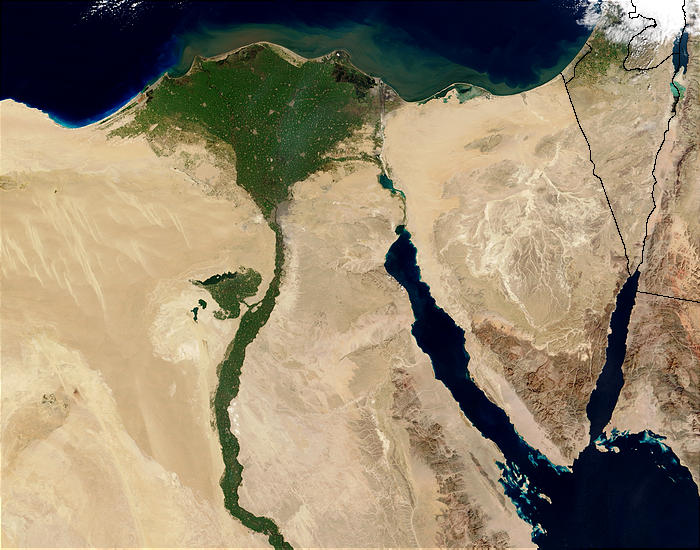
\includegraphics[width=9cm]{nilo}
\end{figure}

Para ejecutar el algoritmo de clasificación, realizamos un total de tres fases:

\textbf{En primer lugar}, aplicamos la técnica de \textbf{apilamiento de enfoque}, el cual consiste en generar a partir de una misma fotografía múltiples imágenes aplicando diferentes enfoques. Para ello disponemos de la función \textit{stack}, disponible en el paquete \textit{raster}.
\begin{Schunk}
\begin{Sinput}
> if(!require(rgdal)){
+   install.packages("rgdal")
+   require(rgdal)
+ }
> # 1. Apilamiento de enfoque
> # Instalamos la libreria
> if(!require(raster)){
+   install.packages("raster")
+   require(raster)
+ }
> # Realizamos el proceso de rasterizado
> image <- stack("nilo.jpg")
\end{Sinput}
\end{Schunk}

\textbf{A continuación}, sobre las imagenes apiladas aplicamos el algoritmo \textit{dbscan} mediante la función \textit{dbscan}, disponible en el paquete \textit{dbscan}. En este caso, ejecutaremos el algoritmo con un total de 10 puntos mínimos para considerar para considerar a una región como un \textit{cluster} (\textbf{minPts}), y una densidad del número de vecinos de 0.8 para cada punto (\textbf{eps}). Analicemos una muestra de los resultados obtenidos:
\begin{footnotesize}
\begin{Schunk}
\begin{Sinput}
> # Incluimos el paquete dbscan
> if(!require(dbscan)){
+   install.packages("dbscan")
+   require(dbscan)
+ }
> db <- dbscan(image[], eps = 0.8, minPts = 10)
> head(db$cluster, 200)
\end{Sinput}
\begin{Soutput}
  [1]  1  2  3  4  5  5  4  4  6  6  6  6  6  6  6  6  7  7  7  7  7  7  7  7  7  7  7  7  7  7  7  7  6  6  6  6  6  6  6  6  6  6  6  6  6  6  6  6  6  6  6  6  6  6  6  6  8  8  8  8  8  8  8  8  8  8  8  8  8  9  9  9 10 10 10 10 10
 [78] 10 10 10 11 11 11 12 12 10 10 10  0  6  0 10 10  0 13  0  0 13 14  0  0  0 13  0  0  0  0  0  0 15  0  0 16 17  0  0  0 10  0  0 18  0  0  0  0  0  0  0  0 19 20 21  0  0 22 22  0 23  0 24  0  0  0 25 23  0 23  0  0 23  0 26  0  0
[155]  0 27 27  0 27 27 12 12 12 12 12 12 12 12 10  0 10 28 10  0 10  0  0 24  0 10 12  0 24 29 29  0  0  0  0 29 29 30  3  3  3  3  3  3  3  3
\end{Soutput}
\end{Schunk}
\end{footnotesize}
Tras ejecutar la función, \textit{dbscan} nos devuelve un \textit{dataframe} con tres campos: \textbf{eps}, \textbf{minPts} y \textbf{cluster}. Este último muestra a qué \textit{cluster} pertenece cada elemento, salvo las filas a 0, los cuales se tratan de \textbf{ruido}.

Para representar los resultados por pantalla \textit{convertimos la imagen original en un conjunto de píxeles}, conocido como \textbf{rasterizado}, utilizando la función \textit{raster}. Finalmente, asignamos cada \textit{cluster} al que pertenece cada punto a cada píxel de la imagen, obteniendo la siguiente imagen:

\begin{figure}[h!]
\centering
\begin{Schunk}
\begin{Sinput}
> # Proceso de rasterizado
> result <- raster(image[[1]])
> # Asignamos el valor del cluster a cada pixel
> result <- setValues(result, db$cluster)
> plot(result)
\end{Sinput}
\end{Schunk}
\includegraphics{G15-P4-046}
\end{figure}
\newpage
Analizando los resultados obtenidos, el algoritmo \textbf{separa correctamente las áreas desérticas con respecto a las zonas con vegetación}. Sin embargo, \textbf{no distingue correctamente entre las zonas de vegetación y el mar}. Esto último puede deberse
a que el número de puntos mínimos sea pequeño, por lo que aumentándolo podríamos llegar a distinguir ligeramente zonas costeras.
\end{document}
